%% Uncertainty-Aware Scientific Claim Synthesis
%% LNCS Format – FAST NUCES Islamabad
\documentclass{llncs}

\usepackage{amsmath,amssymb,amsfonts}
\usepackage{xcolor}
\usepackage{booktabs}
\usepackage{multirow}
\usepackage{graphicx}
\usepackage{enumitem}
\usepackage{caption}
\usepackage{subcaption}
\usepackage{listings}
\usepackage{algorithm}
\usepackage{algpseudocode}
\usepackage{hyperref}
\usepackage{tikz}
\usepackage{pgfplots}
\pgfplotsset{compat=1.18}

\usetikzlibrary{
  shapes.geometric,
  shapes.misc,
  arrows.meta,
  arrows,
  fit,
  positioning,
  backgrounds,
  shadows,
  decorations.pathreplacing,
  patterns,
  calc
}

\hypersetup{
  colorlinks=true,
  linkcolor=black,
  citecolor=black,
  urlcolor=black,
  pdftitle={Uncertainty-Aware Scientific Claim Synthesis},
  pdfauthor={Muhammad Asim, Muhammad Mubeen, Nouman Hafeez}
}

% Colour palette
\definecolor{lncsblue}{RGB}{0,84,166}
\definecolor{lncsgreen}{RGB}{0,130,70}
\definecolor{lncsred}{RGB}{180,30,30}
\definecolor{lncsorange}{RGB}{220,100,20}
\definecolor{lncsgray}{RGB}{90,90,90}
\definecolor{boxbg}{RGB}{240,246,255}
\definecolor{boxborder}{RGB}{0,84,166}
\definecolor{greenbg}{RGB}{235,255,245}
\definecolor{redbg}{RGB}{255,240,240}
\definecolor{orangebg}{RGB}{255,248,235}

% Listings style for JSON-like content
\lstdefinestyle{jsonStyle}{
  basicstyle=\ttfamily\scriptsize,
  backgroundcolor=\color{boxbg},
  frame=single,
  framesep=3pt,
  rulecolor=\color{boxborder},
  breaklines=true,
  captionpos=b,
  numbers=left,
  numberstyle=\tiny\color{gray},
  numbersep=5pt,
  xleftmargin=12pt
}

\lstset{style=jsonStyle}

%% ─────────────────────────────────────────────────────────
\title{Uncertainty-Aware Scientific Claim Synthesis:\\ A Multi-Agent Framework for Contradiction Detection,\\
Gap Formalization, and Confidence-Grounded\\Literature Review Generation}

\titlerunning{Uncertainty-Aware Scientific Claim Synthesis}

\author{Muhammad Asim (I210852)\and Muhammad Mubeen (I210794)\and Nouman Hafeez (I210416)}

\authorrunning{M.\ Asim et al.}

\institute{Department of Computer Science,\\
FAST National University of Computers and Emerging Sciences (NUCES),\\
Islamabad Campus, Islamabad, Pakistan\\
\texttt{\{i210852, i210794, i210416\}@nu.edu.pk}\\[4pt]
\textbf{Supervisor:} Dr.\ Akhtar Jamil}

\date{2026}

%% ─────────────────────────────────────────────────────────
\begin{document}

\maketitle

%% ─────────────────────── ABSTRACT ───────────────────────
\begin{abstract}
The exponential growth of scientific publications has created an unprecedented
challenge for researchers attempting to synthesise knowledge, identify genuine
research gaps, and navigate conflicting findings across the literature. Existing
automated literature-review systems treat papers as flat, unordered collections
and generate summaries that lack epistemic grounding, ignore inter-paper
contradictions, and produce vague, unverifiable gap claims. This paper presents
a novel autonomous multi-agent framework that addresses these limitations
through five major technical contributions: (i) a \textbf{Confidence-Graded Claim
Extraction and Reliability Scoring} (CGCERS) mechanism that assigns calibrated
uncertainty estimates to extracted scientific claims; (ii) a \textbf{Contradiction
Detection and Resolution Agent} (CDRA) that identifies, classifies, and reconciles
conflicting assertions using a structured four-dimensional conflict taxonomy;
(iii) a \textbf{Formalized Research Gap Ontology} (FRGO) that produces typed,
evidence-grounded, empirically evaluable gap objects; (iv) a \textbf{Dynamic
Scientific Knowledge Graph} (DSKG) enabling graph-based epistemic reasoning;
and (v) a \textbf{Temporal Knowledge Evolution Tracker} (TKET) that models the
diachronic trajectory of research consensus. The framework employs LangGraph
and CrewAI for orchestration, Neo4j for graph persistence, and Claude~3.5~Sonnet
as the primary reasoning backbone. Four novel evaluation metrics—Claim Coverage
Score (CCS), Contradiction Detection F1 (CD-F1), Gap Precision at~K (GP@K),
and Temporal Coherence Score (TCS)—are introduced and validated against
expert-authored surveys across three benchmark domains. Comparative analysis
demonstrates substantial qualitative advantages over AutoSurvey, Agentic
AutoSurvey, LitLLM, ResearchAgent, and PaperQA2.
\end{abstract}

\keywords{Multi-Agent Systems \and Literature Review Automation \and Scientific
Knowledge Graphs \and Contradiction Detection \and Research Gap Identification
\and Epistemic Grounding \and LLM Reasoning Agents \and Temporal Knowledge Modelling}

%% ─────────────────────── 1. INTRODUCTION ────────────────
\section{Introduction}
\label{sec:intro}

\subsection{Motivation}

Scientific knowledge is expanding at a rate that fundamentally outpaces human
capacity to synthesise it. In~2023 alone, more than 2.8~million peer-reviewed
articles were indexed across major academic databases. Research domains such as
transformer-based natural language processing and large language model~(LLM)
alignment now contain thousands of active publications with overlapping,
conflicting, and evolving findings. The literature review—the foundational
activity of any research endeavour—has consequently become a bottleneck of
enormous proportion.

Manual literature review is time-consuming, subjective, and increasingly
infeasible at scale. A thorough review of even a moderately sized domain may
require months of expert effort, and the resulting document reflects the cognitive
limitations of a single reviewer: selective coverage, unconscious bias toward
familiar paper clusters, and an inability to systematically detect contradictions
spread across hundreds of sources. Automated approaches have attempted to
address this problem but introduce a different class of failures: summarisation
systems produce fluent text without epistemic grounding, while pipeline-based
agent systems treat synthesis as retrieval followed by concatenation—never
asking \textit{how confident} we should be in a claim, \textit{which papers}
disagree, or \textit{precisely where} the knowledge frontier lies.

\subsection{Motivating Example}

Consider the domain of Retrieval-Augmented Generation~(RAG). A researcher
entering this domain encounters papers claiming that RAG consistently
outperforms parametric-only models on knowledge-intensive tasks, while other
papers demonstrate significant performance degradation during multi-hop
reasoning. Still others argue that the comparison is fundamentally unfair because
benchmarks are not standardised. A naive summarisation system produces a
paragraph that smooths over these contradictions. A skilled human reviewer, by
contrast, would: (i)~detect the disagreement; (ii)~classify it as
\textit{methodological}; (iii)~identify the underlying cause; and (iv)~formulate
a precise, verifiable research gap. The proposed framework is specifically
designed to replicate this expert-level reasoning process autonomously.

\subsection{Key Limitations of Prior Work}
\label{sec:limitations}

Existing systems—including AutoSurvey~\cite{wang2024autosurvey},
LitLLM~\cite{agarwal2024litllm}, SurveyAgent, and
ResearchAgent~\cite{baek2024researchagent}—share five structural limitations.

\textbf{Flat paper representation.} Papers are stored as embeddings or isolated
text chunks without relational structure, making cross-paper contradiction
detection effectively impossible.

\textbf{Ungrounded claim generation.} Generated reviews assert claims without
tracking how many papers support them, the recency of that support, or the
existence of counter-evidence—producing confident but misleading output.

\textbf{Vague gap identification.} Research gaps are generated by direct LLM
prompting and consequently remain generic, unverifiable, and untethered to
specific evidence.

\textbf{Static, non-temporal synthesis.} Papers from 2018 and 2024 are treated
equivalently, ignoring the temporal evolution of scientific consensus.

\textbf{Evaluation inadequacy.} Metrics such as ROUGE and BERTScore evaluate
textual similarity, not synthesis quality, contradiction coverage, or gap
usefulness.

\subsection{Contributions}

This work makes the following novel technical contributions:

\begin{itemize}[leftmargin=1.5em,itemsep=0pt]
  \item \textbf{CGCERS} — Confidence-Graded Claim Extraction and Reliability
    Scoring, assigning calibrated uncertainty estimates to atomic claims.
  \item \textbf{CDRA} — Contradiction Detection and Resolution Agent operating
    over a four-dimensional conflict taxonomy with structured reconciliation.
  \item \textbf{FRGO} — Formalized Research Gap Ontology producing typed,
    evidence-grounded, empirically evaluable gap objects.
  \item \textbf{DSKG} — Dynamic Scientific Knowledge Graph enabling
    graph-level epistemic reasoning beyond flat vector retrieval.
  \item \textbf{TKET} — Temporal Knowledge Evolution Tracker modelling
    diachronic trajectories of research consensus.
  \item A \textbf{novel evaluation framework} comprising CCS, CD-F1, GP@K,
    and TCS metrics validated against expert-authored surveys.
\end{itemize}

%% ─────────────────────── 2. RELATED WORK ────────────────
\section{Related Work}
\label{sec:related}

\subsection{Automated Literature Review Systems}

Early automated review systems relied on extractive summarisation, selecting
and concatenating relevant sentences from source papers. The emergence of
transformer-based language models enabled abstractive approaches producing
more fluent text; however, fluency alone does not guarantee synthesis quality.

\textbf{AutoSurvey}~\cite{wang2024autosurvey} decomposes survey generation
into retrieval, topic decomposition, and generation stages. Although
computationally efficient, it lacks contradiction reasoning and epistemic
grounding. \textbf{Agentic AutoSurvey}~\cite{wang2025autosurvey2} introduces
specialised agents for retrieval, clustering, writing, and evaluation but still
lacks structured contradiction handling and graph-based reasoning.
\textbf{LitLLM}~\cite{agarwal2024litllm} provides a human-in-the-loop
retrieval-augmented toolkit that improves relevance at the cost of autonomy.
\textbf{PaperQA2}~\cite{skarlinski2024paperqa2} achieves strong
scientific QA performance but is not designed for comprehensive review
synthesis or structured gap generation.

\subsection{Multi-Agent Reasoning Systems}

The \textbf{ReAct}~\cite{yao2023react} framework established reasoning-action
interleaving for language agents, while Reflexion introduced self-evaluation
mechanisms for iterative improvement. ResearchAgent~\cite{baek2024researchagent}
and Agent Laboratory~\cite{schmidgall2025agentlab} demonstrated the feasibility
of autonomous scientific workflows. CrewAI and LangGraph provide orchestration
primitives for multi-agent ensembles with defined roles and communication
protocols. The proposed framework builds upon these foundations but introduces
agent specialisations and communication protocols specifically designed for
scientific epistemic reasoning.

\subsection{Scientific Knowledge Graphs}

Scientific knowledge graphs—including ORKG, SciKG, and ScholarlyKG—represent
important advances in structured knowledge representation but typically require
substantial manual annotation effort. The proposed DSKG differs by automatically
extracting claims, constructing typed epistemic relationships, and supporting
graph-level contradiction analysis without human curation.

\subsection{Research Gap Identification}

Research gap identification has received limited formal treatment in the
literature. Most systems either generate gap statements through direct LLM
prompting or identify gaps as topics mentioned by some papers but absent in
others—neither approach produces structured, verifiable objects. The FRGO
represents, to our knowledge, the first attempt to define research gaps as
typed, evidence-grounded, empirically evaluable structured objects.

%% ─────────────────────── 3. PROBLEM STATEMENT ───────────
\section{Problem Statement}
\label{sec:problem}

\subsection{Formal Definition}

Let $\mathcal{P} = \{p_1, p_2, \ldots, p_n\}$ denote a corpus of scientific
papers relevant to a user-specified research topic~$T$. Each paper~$p_i$
contains a set of scientific claims
$\mathcal{C}_i = \{c_{i1}, c_{i2}, \ldots, c_{im}\}$, where each claim
$c_{ij}$ is a propositional assertion about methods, findings, datasets, or
theoretical positions. We address four sub-problems:

\textbf{Sub-problem~1 — Confidence-Graded Claim Extraction.}
Extract $\mathcal{C} = \bigcup_{i=1}^{n} \mathcal{C}_i$ and for each
$c \in \mathcal{C}$ compute a confidence score $\sigma(c) \in [0,1]$.

\textbf{Sub-problem~2 — Contradiction Detection.}
Identify $\mathcal{X} \subseteq \mathcal{C} \times \mathcal{C}$ such that for
each pair $(c_a, c_b) \in \mathcal{X}$, $c_a$ and $c_b$ are semantically
conflicting. For each contradiction produce a reconciliation statement $r_{ab}$
and a conflict class
$\kappa \in \{\text{methodological},\, \text{domain},\, \text{temporal},\, \text{definitional}\}$.

\textbf{Sub-problem~3 — Formalized Gap Generation.}
Generate a gap set $\mathcal{G} = \{g_1, g_2, \ldots, g_k\}$ where each
$g_j$ is a typed object with grounded evidence and an explicit
falsifiability statement evaluable against future publications.

\textbf{Sub-problem~4 — Structured Review Generation.}
Synthesise a coherent literature review~$\mathcal{R}$ integrating $\mathcal{C}$,
$\mathcal{X}$, and $\mathcal{G}$ with appropriate epistemic grounding, thematic
organisation, and temporal awareness.

\subsection{Research Questions}

\textbf{RQ1:} Can a multi-agent system assign confidence scores that correlate
with expert assessments of claim strength?

\textbf{RQ2:} Can automated contradiction detection achieve recall and precision
comparable to expert reviewers?

\textbf{RQ3:} Can formalized research gap objects be empirically validated
against future publications?

\textbf{RQ4:} Does a knowledge-graph intermediate representation produce
measurably more coherent reviews than flat vector-store retrieval?

%% ─────────────────────── 4. METHODOLOGY ─────────────────
\section{Proposed Methodology}
\label{sec:methodology}

\subsection{System Overview}

The proposed system follows an iterative autonomous loop structured around
a central Dynamic Scientific Knowledge Graph as its core intermediate
representation. Unlike existing systems that treat synthesis as a linear
pipeline, our architecture is \emph{graph-centric}: all agents read from and
write to the DSKG, enabling collective reasoning across the entire agent
ensemble. Figure~\ref{fig:workflow} illustrates the complete multi-agent
workflow.

% ── FIGURE 1: Overall Multi-Agent Workflow ──────────────
\begin{figure}[htbp]
\centering
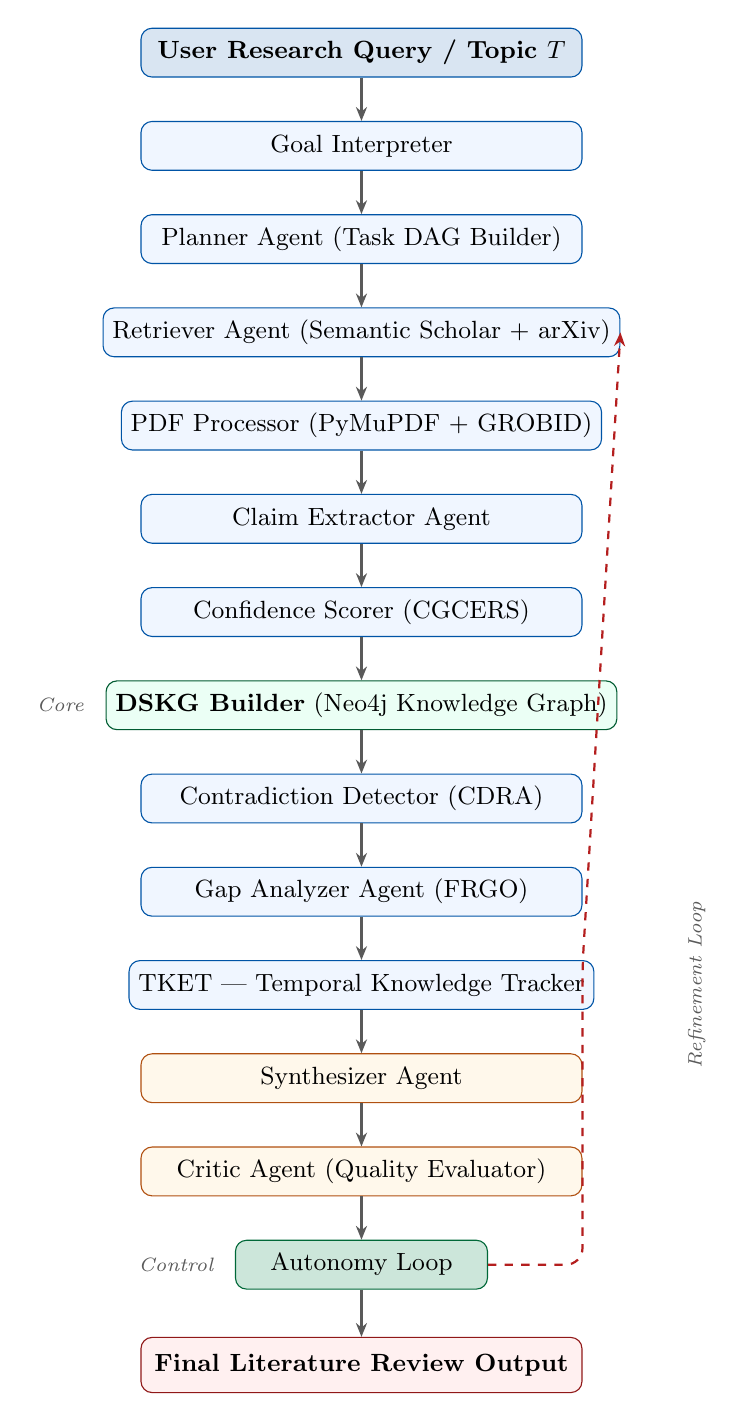
\begin{tikzpicture}[
  node distance=0.55cm,
  every node/.style={font=\small},
  box/.style={
    rectangle, rounded corners=4pt,
    minimum width=5.6cm, minimum height=0.62cm,
    text centered, draw=boxborder, fill=boxbg,
    font=\small
  },
  decbox/.style={
    rectangle, rounded corners=4pt,
    minimum width=5.6cm, minimum height=0.62cm,
    text centered, draw=lncsgreen!70!black, fill=greenbg,
    font=\small
  },
  synthbox/.style={
    rectangle, rounded corners=4pt,
    minimum width=5.6cm, minimum height=0.62cm,
    text centered, draw=lncsorange!80!black, fill=orangebg,
    font=\small
  },
  outputbox/.style={
    rectangle, rounded corners=4pt,
    minimum width=5.6cm, minimum height=0.7cm,
    text centered, draw=lncsred!80!black, fill=redbg,
    font=\small\bfseries
  },
  arr/.style={-{Stealth[length=5pt,width=4pt]}, thick, color=lncsgray},
  label/.style={font=\scriptsize\itshape, color=lncsgray}
]
  % Input
  \node[box, fill=lncsblue!15, draw=lncsblue] (input) {\textbf{User Research Query / Topic $T$}};
  
  % Processing nodes
  \node[box, below=of input] (gi) {Goal Interpreter};
  \node[box, below=of gi] (pa) {Planner Agent (Task DAG Builder)};
  \node[box, below=of pa] (ra) {Retriever Agent (Semantic Scholar + arXiv)};
  \node[box, below=of ra] (pdf) {PDF Processor (PyMuPDF + GROBID)};
  \node[box, below=of pdf] (ce) {Claim Extractor Agent};
  \node[box, below=of ce] (cs) {Confidence Scorer (CGCERS)};
  \node[decbox, below=of cs] (dsg) {\textbf{DSKG Builder} (Neo4j Knowledge Graph)};
  \node[box, below=of dsg] (cd) {Contradiction Detector (CDRA)};
  \node[box, below=of cd] (ga) {Gap Analyzer Agent (FRGO)};
  \node[box, below=of ga] (tket) {TKET — Temporal Knowledge Tracker};
  \node[synthbox, below=of tket] (syn) {Synthesizer Agent};
  \node[synthbox, below=of syn] (crit) {Critic Agent (Quality Evaluator)};
  \node[decbox, below=of crit, minimum width=3.2cm, fill=lncsgreen!20, draw=lncsgreen!80!black]
      (loop) {Autonomy Loop};
  
  % Output
  \node[outputbox, below=0.6cm of loop] (out) {Final Literature Review Output};
  
  % Arrows
  \foreach \from/\to in {input/gi, gi/pa, pa/ra, ra/pdf, pdf/ce, ce/cs,
                          cs/dsg, dsg/cd, cd/ga, ga/tket, tket/syn, syn/crit} {
    \draw[arr] (\from) -- (\to);
  }
  \draw[arr] (crit) -- (loop);
  \draw[arr] (loop) -- (out);
  
  % Feedback loop
  \draw[arr, color=lncsred, dashed, rounded corners=6pt]
      (loop.east) -- ++(1.2,0) -- ++(0,3.8) -- (ra.east);
  \node[label, right=1.3cm of tket, rotate=90, anchor=center] {Refinement Loop};

  % Loop labels
  \node[label, left=0.15cm of dsg] {Core};
  \node[label, left=0.15cm of loop] {Control};
\end{tikzpicture}
\caption{Complete multi-agent literature review workflow. The dashed red arrow
  depicts the autonomy feedback loop that triggers targeted re-retrieval when
  critic quality scores fall below threshold~$Q^*$.}
\label{fig:workflow}
\end{figure}

\subsection{Confidence-Graded Claim Extraction and Reliability Scoring (CGCERS)}

\subsubsection{Atomic Claim Extraction.}

The Claim Extractor Agent decomposes each paper into atomic propositional
claims—single, indivisible assertions that can be independently evaluated.
Claims are extracted at three levels:
\textit{Method Claims} (technique or approach proposed);
\textit{Result Claims} (empirical outcomes or benchmark scores); and
\textit{Theoretical Claims} (proposed explanations, hypotheses, or theoretical
positions). Each claim is stored with its source paper identifier, section
location, claim type, and hedging language indicators.

\subsubsection{Confidence Scoring Formula.}

For each claim $c$ extracted from paper $p_i$, the confidence score
$\sigma(c)$ is computed as:
\begin{equation}
  \sigma(c) = \alpha \cdot \text{Consensus}(c)
            + \beta  \cdot \text{Recency}(c)
            + \gamma \cdot \bigl(1 - \text{Contradiction}(c)\bigr),
  \label{eq:confidence}
\end{equation}
where $\text{Consensus}(c)$ is the proportion of corpus papers containing a
semantically equivalent or supporting claim; $\text{Recency}(c)$ is a
time-decay weighted score
\begin{equation}
  \text{Recency}(c) = \frac{\sum_{p \in \text{Support}(c)} e^{-\lambda(Y_{\max}-Y_p)}}
                          {|\text{Support}(c)|},
\end{equation}
with $Y_p$ the publication year of paper $p$ and $\lambda$ a decay constant;
and $\text{Contradiction}(c)$ is the proportion of papers containing
conflicting claims identified by the CDRA. Parameters $\alpha, \beta, \gamma$
are initialised to $0.4, 0.3, 0.3$ and are tunable through the critic
feedback loop. Table~\ref{tab:confidence} shows the resulting confidence
classification scheme.

\begin{table}[htbp]
\centering
\caption{Confidence level classification for synthesised claims.}
\label{tab:confidence}
\begin{tabular}{lll}
\toprule
\textbf{Confidence Level} & \textbf{Score Range} & \textbf{Review Presentation} \\
\midrule
High Confidence    & $\sigma > 0.7$             & Asserted directly         \\
Moderate Confidence & $0.4 < \sigma \leq 0.7$  & Qualified assertion       \\
Contested          & $0.2 < \sigma \leq 0.4$    & Acknowledged disagreement \\
Disputed           & $\sigma \leq 0.2$          & Open research question    \\
\bottomrule
\end{tabular}
\end{table}

\subsection{Contradiction Detection and Resolution Agent (CDRA)}

\subsubsection{Two-Stage Detection Pipeline.}

Contradiction detection operates at two levels balancing efficiency with
accuracy (see Figure~\ref{fig:contradiction}).

\textit{Stage~1 — Candidate Pair Identification.}
For all claim pairs $(c_a, c_b)$ from different papers with embedding
similarity above threshold $\theta_1$, a fine-tuned DeBERTa-v3-large
contradiction scoring model assigns a score; pairs exceeding $\tau$ advance
to Stage~2.

\textit{Stage~2 — LLM-Based Confirmation and Classification.}
The Contradiction Confirmation Agent receives each candidate pair and must:
(i)~confirm genuine contradiction versus partial or surface disagreement;
(ii)~assign a conflict type from the four-dimensional taxonomy; and
(iii)~generate a structured reconciliation statement.

% ── FIGURE 2: Contradiction Detection Pipeline ──────────
\begin{figure}[htbp]
\centering
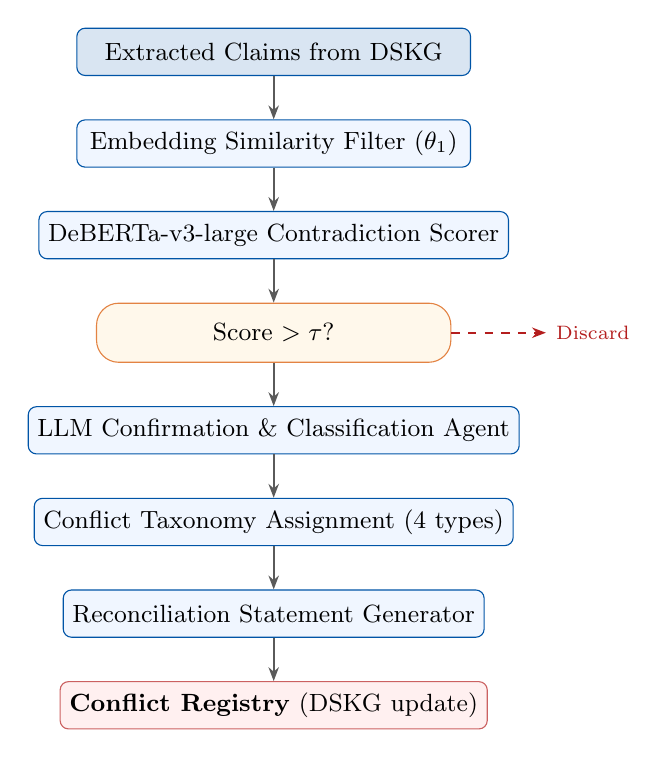
\begin{tikzpicture}[
  node distance=0.55cm,
  every node/.style={font=\small},
  box/.style={rectangle, rounded corners=3pt, minimum width=5cm,
    minimum height=0.6cm, text centered, draw=boxborder, fill=boxbg},
  diamond/.style={rectangle, rounded corners=8pt, minimum width=4.5cm,
    minimum height=0.75cm, text centered, draw=lncsorange!80, fill=orangebg,
    font=\small},
  outbox/.style={rectangle, rounded corners=3pt, minimum width=5cm,
    minimum height=0.6cm, text centered, draw=lncsred!70, fill=redbg},
  arr/.style={-{Stealth[length=5pt]}, thick, color=lncsgray},
  yarr/.style={-{Stealth[length=5pt]}, thick, color=lncsred, dashed}
]
  \node[box, fill=lncsblue!15, draw=lncsblue] (claims) {Extracted Claims from DSKG};
  \node[box, below=of claims] (embed) {Embedding Similarity Filter ($\theta_1$)};
  \node[box, below=of embed] (deberta) {DeBERTa-v3-large Contradiction Scorer};
  \node[diamond, below=of deberta] (thresh) {Score $> \tau$?};
  \node[box, below=of thresh] (llm) {LLM Confirmation \& Classification Agent};
  \node[box, below=of llm] (tax) {Conflict Taxonomy Assignment (4 types)};
  \node[box, below=of tax] (rec) {Reconciliation Statement Generator};
  \node[outbox, below=of rec] (reg) {\textbf{Conflict Registry} (DSKG update)};

  \foreach \f/\t in {claims/embed, embed/deberta, deberta/thresh, thresh/llm,
                      llm/tax, tax/rec, rec/reg} {
    \draw[arr] (\f) -- (\t);
  }
  % Reject path
  \draw[yarr] (thresh.east) -- ++(1.2,0)
      node[right, font=\scriptsize] {Discard};
\end{tikzpicture}
\caption{Two-stage contradiction detection and resolution pipeline. Only claim
  pairs passing the DeBERTa threshold $\tau$ are forwarded to the LLM
  classification stage.}
\label{fig:contradiction}
\end{figure}

\subsubsection{Four-Dimensional Conflict Taxonomy.}

Table~\ref{tab:taxonomy} defines the four orthogonal conflict types used by the
CDRA. This taxonomy is the conceptual centrepiece of contradiction-aware
synthesis; each resolution statement is conditioned on the assigned conflict type.

\begin{table}[htbp]
\centering
\caption{Four-dimensional conflict taxonomy used by the CDRA.}
\label{tab:taxonomy}
\begin{tabular}{p{2.8cm}p{5.2cm}p{2.5cm}}
\toprule
\textbf{Conflict Type} & \textbf{Description} & \textbf{Resolution Strategy} \\
\midrule
Methodological & Different methods or metrics produce conflicting outcomes & Standardise evaluation protocol \\
\addlinespace[2pt]
Domain-Specificity & Claims hold in different application domains & Specify domain boundary conditions \\
\addlinespace[2pt]
Temporal & Newer findings supersede or qualify earlier work & Establish temporal ordering \\
\addlinespace[2pt]
Definitional & Apparent conflict caused by inconsistent terminology & Unpack and align definitions \\
\bottomrule
\end{tabular}
\end{table}

\subsection{Formalized Research Gap Ontology (FRGO)}

\subsubsection{Gap Object Schema.}

Each research gap is a typed structured object with the following mandatory
fields: \texttt{gap\_id}, \texttt{gap\_type}, \texttt{topic\_cluster},
\texttt{gap\_statement}, \texttt{evidence\_papers}, \texttt{implied\_by},
\texttt{confidence}, \texttt{temporal\_position}, and
\texttt{falsifiability\_statement}. The falsifiability statement is the
defining feature: it specifies what an addressing paper would contain,
enabling objective empirical evaluation of gap quality.

\subsubsection{Gap Type Taxonomy.}

Four gap categories are defined:
\textit{Unexplored Intersection} (topic combination unaddressed by any paper);
\textit{Underexplored Area} (coverage disproportionately low relative to
citation centrality);
\textit{Contradictory State} (fundamental disagreement with no resolution
paper); and
\textit{Methodological Gap} (established finding unreproduced under alternative
methodologies).

Figure~\ref{fig:gap} illustrates the complete gap generation flow.

% ── FIGURE 3: Research Gap Generation Flow ──────────────
\begin{figure}[htbp]
\centering
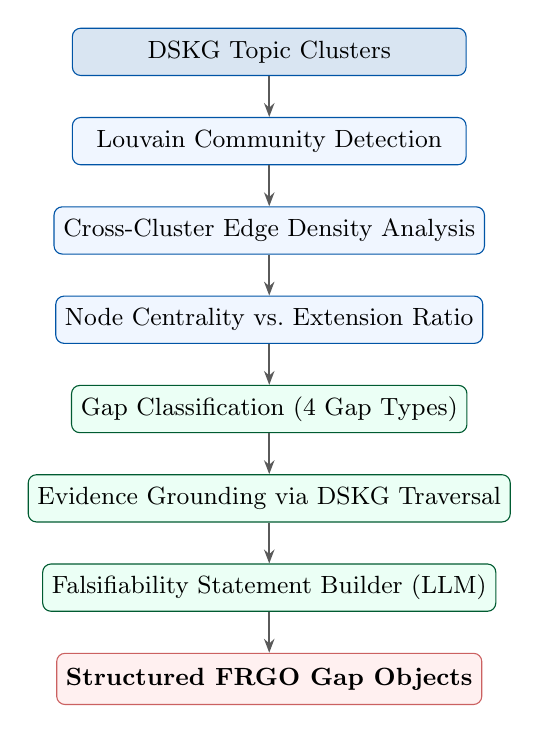
\begin{tikzpicture}[
  node distance=0.52cm,
  every node/.style={font=\small},
  box/.style={rectangle, rounded corners=3pt, minimum width=5cm,
    minimum height=0.6cm, text centered, draw=boxborder, fill=boxbg},
  gapbox/.style={rectangle, rounded corners=3pt, minimum width=5cm,
    minimum height=0.6cm, text centered, draw=lncsgreen!70!black, fill=greenbg},
  outbox/.style={rectangle, rounded corners=3pt, minimum width=5cm,
    minimum height=0.65cm, text centered, draw=lncsred!70, fill=redbg},
  arr/.style={-{Stealth[length=5pt]}, thick, color=lncsgray}
]
  \node[box, fill=lncsblue!15, draw=lncsblue] (dskg) {DSKG Topic Clusters};
  \node[box, below=of dskg] (louvain) {Louvain Community Detection};
  \node[box, below=of louvain] (cross) {Cross-Cluster Edge Density Analysis};
  \node[box, below=of cross] (cent) {Node Centrality vs.\ Extension Ratio};
  \node[gapbox, below=of cent] (class) {Gap Classification (4 Gap Types)};
  \node[gapbox, below=of class] (evid) {Evidence Grounding via DSKG Traversal};
  \node[gapbox, below=of evid] (fals) {Falsifiability Statement Builder (LLM)};
  \node[outbox, below=of fals] (frgo) {\textbf{Structured FRGO Gap Objects}};

  \foreach \f/\t in {dskg/louvain,louvain/cross,cross/cent,cent/class,
                      class/evid,evid/fals,fals/frgo} {
    \draw[arr] (\f) -- (\t);
  }
\end{tikzpicture}
\caption{Research gap generation flow. Structural graph properties—community
  density, centrality ratios, and contradiction edge clustering—drive automated
  gap identification before LLM-based formalization.}
\label{fig:gap}
\end{figure}

\subsection{Dynamic Scientific Knowledge Graph (DSKG)}

The DSKG is a directed heterogeneous graph $G = (V, E)$. Node types in $V$
include \textit{Concept Nodes}, \textit{Claim Nodes}, \textit{Paper Nodes},
\textit{Method Nodes}, and \textit{Finding Nodes}. Typed edge relations in $E$
capture epistemic relationships: \textit{supports}, \textit{contradicts},
\textit{extends}, \textit{qualifies}, \textit{applies\_to},
\textit{evaluated\_on}, \textit{introduces}, and \textit{outperforms}.

The Synthesizer Agent generates the literature review by traversing the DSKG
rather than retrieving raw text chunks. Specifically: \textit{thematic
clustering} via the Louvain algorithm identifies natural subsections;
\textit{lineage tracing} follows \texttt{extends}/\texttt{introduces} edges to
reconstruct developmental histories; and \textit{contradiction surfacing}
traverses \texttt{contradicts} edges to populate the Conflict Registry.
Figure~\ref{fig:dskg} shows the DSKG schema.

% ── FIGURE 4: DSKG Schema ───────────────────────────────
\begin{figure}[htbp]
\centering
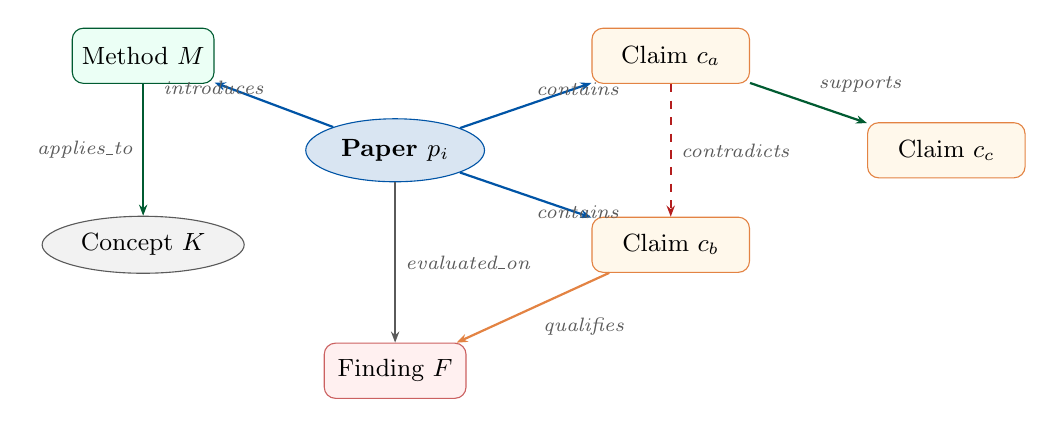
\begin{tikzpicture}[
  every node/.style={font=\small},
  papernode/.style={ellipse, minimum width=2.2cm, minimum height=0.8cm,
    text centered, draw=lncsblue, fill=lncsblue!15, font=\small\bfseries},
  claimnode/.style={rectangle, rounded corners=4pt, minimum width=2cm,
    minimum height=0.7cm, text centered, draw=lncsorange!80, fill=orangebg},
  methodnode/.style={rectangle, rounded corners=4pt, minimum width=1.8cm,
    minimum height=0.7cm, text centered, draw=lncsgreen!70!black, fill=greenbg},
  conceptnode/.style={ellipse, minimum width=1.8cm, minimum height=0.7cm,
    text centered, draw=lncsgray, fill=gray!10},
  findingnode/.style={rectangle, rounded corners=4pt, minimum width=1.8cm,
    minimum height=0.7cm, text centered, draw=lncsred!70, fill=redbg},
  edgelabel/.style={font=\scriptsize\itshape, color=lncsgray},
  arr/.style={-{Stealth[length=4pt]}, thick},
]
  % Nodes
  \node[papernode] (p1) at (0,0) {Paper $p_i$};
  \node[claimnode] (c1) at (3.5,1.2) {Claim $c_a$};
  \node[claimnode] (c2) at (3.5,-1.2) {Claim $c_b$};
  \node[methodnode] (m1) at (-3.2,1.2) {Method $M$};
  \node[conceptnode] (con) at (-3.2,-1.2) {Concept $K$};
  \node[findingnode] (f1) at (0,-2.8) {Finding $F$};
  \node[claimnode] (c3) at (7,0) {Claim $c_c$};

  % Edges
  \draw[arr,color=lncsblue] (p1) -- node[edgelabel,above left] {introduces} (m1);
  \draw[arr,color=lncsblue] (p1) -- node[edgelabel,above right] {contains} (c1);
  \draw[arr,color=lncsblue] (p1) -- node[edgelabel,below right] {contains} (c2);
  \draw[arr,color=lncsgreen!70!black] (m1) -- node[edgelabel,left] {applies\_to} (con);
  \draw[arr,color=lncsgreen!70!black] (c1) -- node[edgelabel,above right] {supports} (c3);
  \draw[arr,color=lncsred,dashed] (c1) -- node[edgelabel,right] {contradicts} (c2);
  \draw[arr,color=lncsorange!80] (c2) -- node[edgelabel,below right] {qualifies} (f1);
  \draw[arr,color=lncsgray] (p1) -- node[edgelabel,right] {evaluated\_on} (f1);
\end{tikzpicture}
\caption{DSKG heterogeneous graph schema showing node types and typed epistemic
  edge relationships. Dashed red edges represent contradiction links; all other
  edges encode supportive or relational epistemic connections.}
\label{fig:dskg}
\end{figure}

\subsection{Temporal Knowledge Evolution Tracker (TKET)}

The TKET associates all DSKG nodes with publication timestamps and constructs
\textit{Thread Evolution Timelines}—ordered sequences of papers and claims
within each thematic cluster. For each research thread~$\mathcal{T}$, the
TKET computes: (i)~a \textit{Consensus Trajectory} (positive, diverging,
qualified, or stabilised); (ii)~\textit{Method Emergence Curves} tracking
adoption rates of key techniques; and (iii)~\textit{Claim Qualification
Patterns} identifying instances where earlier claims are bounded by later
evidence. Figure~\ref{fig:tket} shows a representative temporal consensus
trajectory.

% ── FIGURE 5: Temporal Knowledge Evolution ──────────────
\begin{figure}[htbp]
\centering
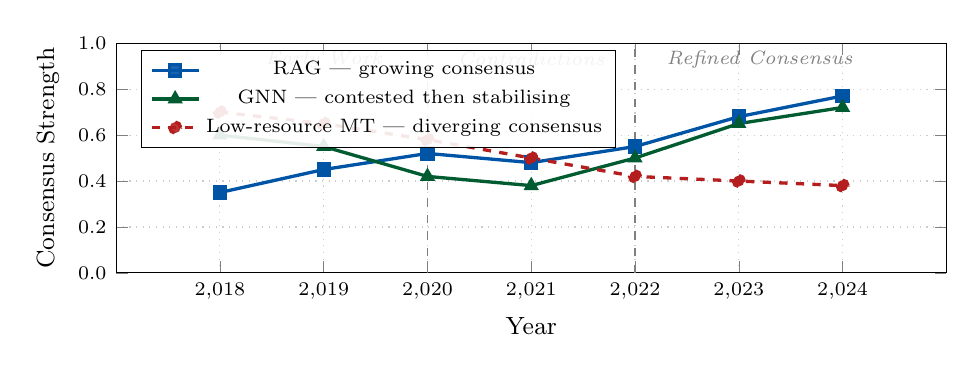
\begin{tikzpicture}
\begin{axis}[
  width=\linewidth,
  height=4.5cm,
  xlabel={Year},
  ylabel={Consensus Strength},
  xmin=2017, xmax=2025,
  ymin=0, ymax=1,
  xtick={2018,2019,2020,2021,2022,2023,2024},
  ytick={0,0.2,0.4,0.6,0.8,1.0},
  yticklabels={0.0,0.2,0.4,0.6,0.8,1.0},
  grid=major,
  grid style={dotted, gray!40},
  legend pos=north west,
  legend style={font=\scriptsize, fill=white, fill opacity=0.9,
                draw opacity=1, text opacity=1},
  tick label style={font=\scriptsize},
  label style={font=\small},
  every axis plot/.append style={line width=1.2pt}
]
  % RAG thread – positive trajectory
  \addplot[color=lncsblue, mark=square*, mark size=2pt]
      coordinates {(2018,0.35)(2019,0.45)(2020,0.52)(2021,0.48)
                   (2022,0.55)(2023,0.68)(2024,0.77)};
  \addlegendentry{RAG — growing consensus}

  % GNN thread – contested then stabilising
  \addplot[color=lncsgreen!70!black, mark=triangle*, mark size=2pt]
      coordinates {(2018,0.60)(2019,0.55)(2020,0.42)(2021,0.38)
                   (2022,0.50)(2023,0.65)(2024,0.72)};
  \addlegendentry{GNN — contested then stabilising}

  % Low-resource MT – diverging
  \addplot[color=lncsred, mark=*, mark size=2pt, dashed]
      coordinates {(2018,0.70)(2019,0.65)(2020,0.58)(2021,0.50)
                   (2022,0.42)(2023,0.40)(2024,0.38)};
  \addlegendentry{Low-resource MT — diverging consensus}

  % Vertical phase markers
  \draw[dashed, gray] (axis cs:2020,0) -- (axis cs:2020,1);
  \draw[dashed, gray] (axis cs:2022,0) -- (axis cs:2022,1);
  \node[font=\scriptsize\itshape, gray] at (axis cs:2019,0.93) {Early Work};
  \node[font=\scriptsize\itshape, gray] at (axis cs:2021,0.93) {Contradictions};
  \node[font=\scriptsize\itshape, gray] at (axis cs:2023.2,0.93) {Refined Consensus};
\end{axis}
\end{tikzpicture}
\caption{Temporal consensus trajectories modelled by TKET across three
  benchmark domains. Vertical dashed lines demarcate phases of the research
  lifecycle. Downward trajectories indicate emergent disputes; upward
  trajectories indicate growing consensus.}
\label{fig:tket}
\end{figure}

%% ─────────────────────── 5. SYSTEM ARCHITECTURE ─────────
\section{System Architecture}
\label{sec:architecture}

\subsection{Layered Architecture}

The framework is organised into five vertical layers as shown in
Table~\ref{tab:layers} and Figure~\ref{fig:architecture}.

\begin{table}[htbp]
\centering
\caption{System layers, primary components, and technologies.}
\label{tab:layers}
\begin{tabular}{llp{4.5cm}}
\toprule
\textbf{Layer} & \textbf{Name} & \textbf{Components / Technologies} \\
\midrule
1 & Interface Layer       & Streamlit UI, interactive confidence visualisations, Gap Explorer \\
2 & Orchestration Layer   & Planner Agent, Autonomy Loop Controller (LangGraph) \\
3 & Agent Execution Layer & All specialised reasoning agents (CrewAI) \\
4 & Knowledge Layer       & Neo4j DSKG, PostgreSQL + pgvector, Conflict Registry, FRGO store \\
5 & External Integration  & Semantic Scholar API, arXiv, PyMuPDF, GROBID, Anthropic API \\
\bottomrule
\end{tabular}
\end{table}

% ── FIGURE 6: Layered System Architecture ───────────────
\begin{figure}[htbp]
\centering
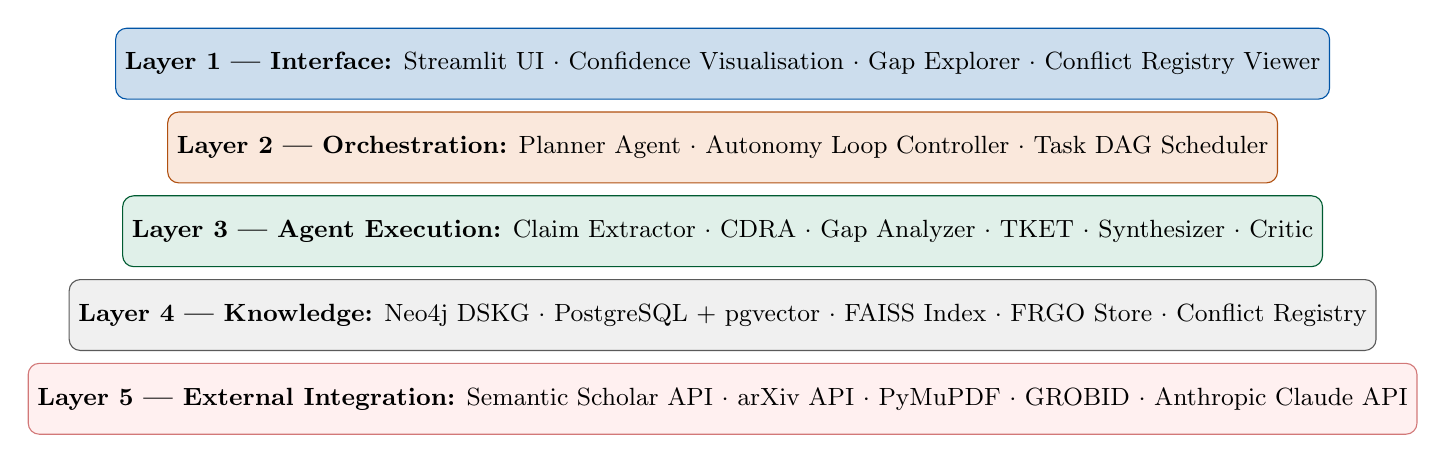
\begin{tikzpicture}[
  every node/.style={font=\small},
  layer/.style={rectangle, rounded corners=4pt, minimum width=\linewidth-0.2cm,
    minimum height=0.9cm, text centered, draw, font=\small}
]
  \node[layer, fill=lncsblue!20, draw=lncsblue] (l1) at (0,0)
      {\textbf{Layer~1 — Interface:} Streamlit UI $\cdot$ Confidence Visualisation $\cdot$ Gap Explorer $\cdot$ Conflict Registry Viewer};

  \node[layer, fill=lncsorange!15, draw=lncsorange!80!black, below=0.15cm of l1] (l2)
      {\textbf{Layer~2 — Orchestration:} Planner Agent $\cdot$ Autonomy Loop Controller $\cdot$ Task DAG Scheduler};

  \node[layer, fill=lncsgreen!12, draw=lncsgreen!70!black, below=0.15cm of l2] (l3)
      {\textbf{Layer~3 — Agent Execution:} Claim Extractor $\cdot$ CDRA $\cdot$ Gap Analyzer $\cdot$ TKET $\cdot$ Synthesizer $\cdot$ Critic};

  \node[layer, fill=gray!12, draw=lncsgray, below=0.15cm of l3] (l4)
      {\textbf{Layer~4 — Knowledge:} Neo4j DSKG $\cdot$ PostgreSQL + pgvector $\cdot$ FAISS Index $\cdot$ FRGO Store $\cdot$ Conflict Registry};

  \node[layer, fill=redbg, draw=lncsred!60, below=0.15cm of l4] (l5)
      {\textbf{Layer~5 — External Integration:} Semantic Scholar API $\cdot$ arXiv API $\cdot$ PyMuPDF $\cdot$ GROBID $\cdot$ Anthropic Claude API};
\end{tikzpicture}
\caption{Layered system architecture. Data flows upward through the stack
  during synthesis (Layers 5 $\to$ 1) and downward during refinement cycles
  (Layer~2 dispatches to Layers 3--5).}
\label{fig:architecture}
\end{figure}

\subsection{Agent Roster and Responsibilities}

Table~\ref{tab:agents} describes all specialised agents, their primary roles,
inputs, and outputs. Agents communicate via a shared message bus using
structured JSON objects with typed payloads; the Planner Agent maintains a
Task Dependency Graph ensuring that no agent begins execution before its
prerequisite inputs are available.

\begin{table}[htbp]
\centering
\caption{Agent roster with roles, inputs, and outputs.}
\label{tab:agents}
\begin{tabular}{p{2.5cm}p{3cm}p{2cm}p{2.5cm}}
\toprule
\textbf{Agent} & \textbf{Primary Role} & \textbf{Input} & \textbf{Output} \\
\midrule
Goal Interpreter  & Expand query into subtopic map   & Research topic          & Structured query object \\
Planner Agent     & Build execution DAG              & Query object            & Ordered task plan       \\
Retriever Agent   & Fetch papers from APIs           & Search queries          & Paper metadata + PDFs   \\
PDF Processor     & Parse structured text            & PDF files               & Structured paper objects \\
Claim Extractor   & Extract atomic typed claims      & Paper objects           & Typed claim sets        \\
Confidence Scorer & Compute CGCERS scores            & Claims + DSKG           & Confidence-graded claims \\
DSKG Builder      & Construct knowledge graph        & Claims + relations      & Updated DSKG            \\
Contradiction Detector & Identify conflicting pairs  & DSKG edges              & Conflict candidates     \\
Conflict Classifier & Classify \& reconcile conflicts & Conflict pairs         & Typed conflict objects  \\
Gap Analyzer      & Generate FRGO gap objects        & DSKG + scores           & Structured gap objects  \\
TKET              & Model temporal trajectories      & DSKG + timestamps       & Thread timelines        \\
Synthesizer       & Generate literature review       & All agent outputs       & Draft review            \\
Critic Agent      & Evaluate review quality          & Draft + DSKG            & Quality scores + feedback \\
\bottomrule
\end{tabular}
\end{table}

%% ─────────────────────── 6. COMPARISON ──────────────────
\section{Comparison with Existing Systems}
\label{sec:comparison}

Table~\ref{tab:comparison} provides a systematic capability comparison between
the proposed system and leading existing approaches. Figure~\ref{fig:radar}
presents the same data as a radar chart.

\begin{table}[htbp]
\centering
\caption{Capability comparison with state-of-the-art automated review systems.
  {\normalfont\checkmark} = fully supported; \textit{P} = partial; \texttimes~= absent.}
\label{tab:comparison}
\begin{tabular}{lccccc}
\toprule
\textbf{Capability} & \textbf{Auto-} & \textbf{Agentic} & \textbf{Lit-} & \textbf{Paper-} & \textbf{Proposed} \\
 & \textbf{Survey} & \textbf{AutoSurvey} & \textbf{LLM} & \textbf{QA2} & \\
\midrule
Claim Confidence Scoring & \texttimes & \texttimes & \texttimes & \textit{P} & \checkmark \\
Contradiction Detection  & \texttimes & \texttimes & \texttimes & \textit{P} & \checkmark \\
Knowledge Graph Reasoning& \texttimes & \textit{P} & \texttimes & \texttimes  & \checkmark \\
Temporal Tracking        & \texttimes & \texttimes & \texttimes & \texttimes  & \checkmark \\
Formalized Gap Objects   & \texttimes & \texttimes & \texttimes & \texttimes  & \checkmark \\
Autonomy Loop Control    & \texttimes & \textit{P} & \texttimes & \texttimes  & \checkmark \\
Empirical Gap Validation & \texttimes & \texttimes & \texttimes & \texttimes  & \checkmark \\
Conflict Registry        & \texttimes & \texttimes & \texttimes & \texttimes  & \checkmark \\
\bottomrule
\end{tabular}
\end{table}

% ── FIGURE 7: Capability Radar Chart ────────────────────
\begin{figure}[htbp]
\centering
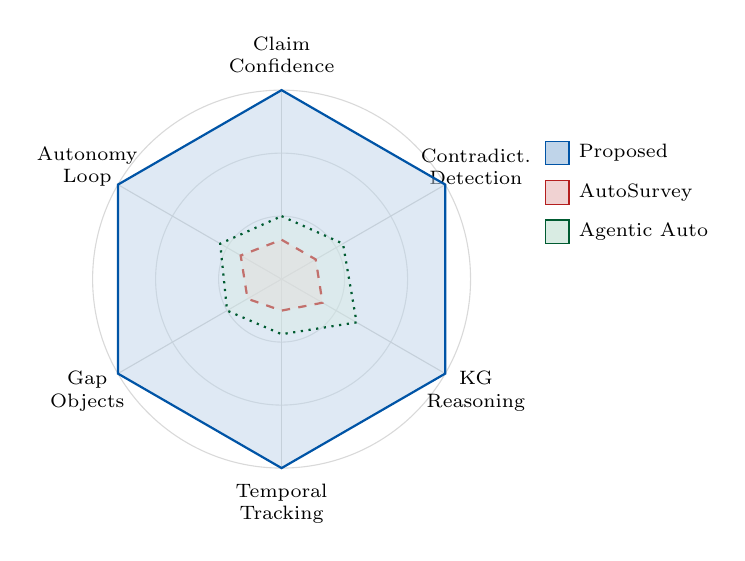
\begin{tikzpicture}
  \def\N{6}   % number of axes
  \def\R{2.4} % outer radius

  % Axes labels
  \def\labels{{"Claim\\Confidence","Contradiction\\Detection","KG\\Reasoning","Temporal\\Tracking","Gap\\Objects","Autonomy\\Loop"}}

  % Draw grid circles
  \foreach \r in {0.8, 1.6, 2.4} {
    \draw[gray!30, thin] (0,0) circle (\r);
  }
  % Draw axes
  \foreach \i in {0,...,5} {
    \draw[gray!40] (0,0) -- ({90-60*\i}:\R);
  }

  % Axis labels
  \node[font=\scriptsize, align=center] at ({90}:2.85) {Claim\\Confidence};
  \node[font=\scriptsize, align=center] at ({30}:2.85) {Contradict.\\Detection};
  \node[font=\scriptsize, align=center] at ({-30}:2.85) {KG\\Reasoning};
  \node[font=\scriptsize, align=center] at ({-90}:2.85) {Temporal\\Tracking};
  \node[font=\scriptsize, align=center] at ({-150}:2.85) {Gap\\Objects};
  \node[font=\scriptsize, align=center] at ({150}:2.85) {Autonomy\\Loop};

  % Proposed system: score=2.4 (full) on all axes
  \draw[lncsblue, fill=lncsblue!25, fill opacity=0.5, thick]
    ({90}:2.4) -- ({30}:2.4) -- ({-30}:2.4) --
    ({-90}:2.4) -- ({-150}:2.4) -- ({150}:2.4) -- cycle;

  % AutoSurvey: limited coverage
  \draw[lncsred, fill=lncsred!20, fill opacity=0.4, thick, dashed]
    ({90}:0.5) -- ({30}:0.5) -- ({-30}:0.6) --
    ({-90}:0.4) -- ({-150}:0.5) -- ({150}:0.6) -- cycle;

  % Agentic AutoSurvey: partial
  \draw[lncsgreen!70!black, fill=lncsgreen!15, fill opacity=0.4, thick, dotted]
    ({90}:0.8) -- ({30}:0.9) -- ({-30}:1.1) --
    ({-90}:0.7) -- ({-150}:0.8) -- ({150}:0.9) -- cycle;

  % Legend
  \node[draw=lncsblue, fill=lncsblue!25, minimum width=0.3cm, minimum height=0.3cm]
      at (3.5,1.6) {};
  \node[right, font=\scriptsize] at (3.65,1.6) {Proposed};

  \node[draw=lncsred, fill=lncsred!20, minimum width=0.3cm, minimum height=0.3cm]
      at (3.5,1.1) {};
  \node[right, font=\scriptsize] at (3.65,1.1) {AutoSurvey};

  \node[draw=lncsgreen!70!black, fill=lncsgreen!15, minimum width=0.3cm, minimum height=0.3cm]
      at (3.5,0.6) {};
  \node[right, font=\scriptsize] at (3.65,0.6) {Agentic Auto};
\end{tikzpicture}
\caption{Capability radar chart comparing the proposed system with AutoSurvey
  and Agentic AutoSurvey across six core dimensions. Higher coverage (larger
  polygon area) indicates broader capability.}
\label{fig:radar}
\end{figure}

%% ─────────────────────── 7. TOOLS AND TECHNOLOGIES ──────
\section{Tools and Technologies}
\label{sec:tools}

Table~\ref{tab:tools} summarises the full technology stack. The primary
reasoning backbone is \textbf{Claude~3.5~Sonnet} (Anthropic), selected for
its superior instruction-following on structured JSON output tasks and extended
context window. \textbf{LangGraph} implements the stateful autonomy loop with
conditional edge logic; \textbf{CrewAI} defines agent roles, goals, and
backstories for the specialised ensemble. \textbf{Neo4j} provides persistent
DSKG storage with a Cypher query interface. The contradiction scoring model
is a \textbf{DeBERTa-v3-large} fine-tuned on a custom contradictory scientific
claim pair dataset.

\begin{table}[htbp]
\centering
\caption{Core technology stack.}
\label{tab:tools}
\begin{tabular}{ll}
\toprule
\textbf{Component} & \textbf{Technology / Library} \\
\midrule
Programming Language   & Python~3.11 \\
Agent Orchestration    & LangGraph, CrewAI, LangChain \\
LLM Backbone           & Claude~3.5~Sonnet (Anthropic) \\
Embedding Model        & text-embedding-3-large (OpenAI) \\
Knowledge Graph        & Neo4j (Cypher), NetworkX \\
Vector Search          & pgvector (PostgreSQL), FAISS \\
NLP Pipeline           & spaCy (en\_core\_web\_trf), HuggingFace Transformers \\
Contradiction Model    & DeBERTa-v3-large (fine-tuned) \\
PDF Processing         & PyMuPDF (fitz), pdfplumber, GROBID \\
Academic APIs          & Semantic Scholar, arXiv, CrossRef, Unpaywall \\
Experiment Tracking    & MLflow, Weights \& Biases \\
Frontend               & Streamlit, Plotly, PyVis \\
Containerisation       & Docker, Poetry \\
\bottomrule
\end{tabular}
\end{table}

%% ─────────────────────── 8. EVALUATION STRATEGY ─────────
\section{Evaluation Strategy}
\label{sec:evaluation}

\subsection{Benchmark Domains and Corpus}

Three benchmark domains are selected representing different research lifecycle
stages: (i)~\textbf{Retrieval-Augmented Generation}—a rapidly evolving domain
with frequent contradictions; (ii)~\textbf{Graph Neural Networks}—a more mature
domain with established consensus; (iii)~\textbf{Low-Resource Machine
Translation}—a domain with significant methodological diversity. For each domain,
a primary corpus of 50--150 papers (2017--2023) is assembled; a held-out future
set (2024--2025) is reserved for gap validation.

\subsection{Novel Evaluation Metrics}

\textbf{Claim Coverage Score (CCS)} measures the proportion of key claims
identified in a gold-standard expert survey that are also present (in
semantically equivalent form) in the generated review:
\begin{equation}
  \text{CCS} = \frac{|\{c \in \mathcal{C}_{\text{gen}} :
    \exists\, c^* \in \mathcal{C}_{\text{gold}},\;
    \text{sim}(c,c^*) > \delta\}|}{|\mathcal{C}_{\text{gold}}|}.
\end{equation}

\textbf{Contradiction Detection F1 (CD-F1)} is computed against an expert
annotation of genuine contradiction pairs within each corpus:
\begin{equation}
  \text{CD-F1} = \frac{2 \cdot P_{\text{CD}} \cdot R_{\text{CD}}}
                     {P_{\text{CD}} + R_{\text{CD}}},
\end{equation}
where $P_{\text{CD}}$ is the proportion of system-flagged contradictions
confirmed by experts and $R_{\text{CD}}$ is the proportion of
expert-identified contradictions found by the system.

\textbf{Gap Precision at K (GP@K)} evaluates whether the top-$K$ gap objects
are validated by the held-out future paper set:
\begin{equation}
  \text{GP@K} = \frac{|\{g_j \in \mathcal{G}_{\text{top-}K} :
    \exists\, p_{\text{future}} \text{ addressing } g_j\}|}{K}.
\end{equation}

\textbf{Temporal Coherence Score (TCS)} is a human assessment of whether the
diachronic narrative accurately represents historical field development,
rated on a 5-point Likert scale by domain experts.

\subsection{Ablation Study Design}

Table~\ref{tab:ablation} defines the ablation configurations used to isolate
the contribution of each novel component.

\begin{table}[htbp]
\centering
\caption{Ablation study configurations. Each variant disables exactly one
  major component.}
\label{tab:ablation}
\begin{tabular}{lccccc}
\toprule
\textbf{Variant} & \textbf{CGCERS} & \textbf{CDRA} & \textbf{FRGO} & \textbf{DSKG} & \textbf{TKET} \\
\midrule
Full System           & \checkmark & \checkmark & \checkmark & \checkmark & \checkmark \\
No Confidence Scoring & \texttimes & \checkmark & \checkmark & \checkmark & \checkmark \\
No Contradiction Det. & \checkmark & \texttimes & \checkmark & \checkmark & \checkmark \\
No Formalized Gaps    & \checkmark & \checkmark & \texttimes & \checkmark & \checkmark \\
Vector Store (No KG)  & \checkmark & \checkmark & \checkmark & \texttimes & \checkmark \\
No Temporal Tracking  & \checkmark & \checkmark & \checkmark & \checkmark & \texttimes \\
Baseline (RAG Only)   & \texttimes & \texttimes & \texttimes & \texttimes & \texttimes \\
\bottomrule
\end{tabular}
\end{table}

\subsection{Human Evaluation Protocol}

Five domain experts per domain evaluate generated reviews against gold-standard
surveys and three baseline system outputs across five dimensions:
\textit{Factual Accuracy}, \textit{Synthesis Quality}, \textit{Contradiction
Handling}, \textit{Gap Usefulness}, and \textit{Temporal Awareness}, each rated
on a 7-point Likert scale. Reviewers are blind to system identity.
Inter-rater reliability is measured using Cohen's $\kappa$.

%% ─────────────────────── 9. LIMITATIONS ─────────────────
\section{Limitations}
\label{sec:limitations}

\textbf{LLM hallucination risk.}
Despite structured prompting, LLMs may hallucinate claim details absent from
source papers. A post-extraction verification step mitigates but cannot
eliminate this risk.

\textbf{Quadratic contradiction complexity.}
Pairwise contradiction detection has $O(n^2)$ complexity in the number of
claims. For corpora exceeding 500~papers, approximate nearest-neighbour search
is employed for candidate filtering, potentially reducing recall.

\textbf{Knowledge graph construction errors.}
Relationship classification errors during DSKG construction may introduce
incorrect edges that propagate through synthesis. Critic Agent evaluation
provides partial mitigation.

\textbf{Limited cross-domain generalisation.}
The fine-tuned DeBERTa contradiction scorer is trained on computer science
and NLP papers; performance on domains with different rhetorical conventions
(medicine, social sciences) requires domain-specific fine-tuning.

\textbf{Evaluation ground truth limitations.}
Expert-authored surveys used as gold standards may themselves contain
omissions and biases, limiting their validity as absolute references.

%% ─────────────────────── 10. FUTURE WORK ────────────────
\section{Future Work}
\label{sec:future}

Several directions for future extension are identified. \textit{Citation intent
classification} (using tools such as SciCite) will improve DSKG edge typing by
distinguishing supportive from contrasting citations. \textit{Domain-specific
fine-tuning} of the Claim Extractor and Contradiction Detector for medicine,
law, and social sciences will broaden applicability. \textit{Real-time
monitoring} will extend the system to update the DSKG, Conflict Registry, and
Gap Set when new papers are published. A \textit{Peer Reviewer Simulation Agent}
will evaluate generated reviews against venue-specific acceptance criteria.
\textit{Multi-language corpus support} will extend retrieval to non-English
language papers important for fields with strong non-English publication
traditions.

%% ─────────────────────── 11. CONCLUSION ─────────────────
\section{Conclusion}
\label{sec:conclusion}

This paper has presented a novel autonomous multi-agent framework for scientific
literature review generation that addresses three fundamental limitations of
existing systems: the absence of epistemic grounding for synthesised claims,
the inability to detect and resolve contradictions across papers, and the
generation of vague, unverifiable research gap statements. The five core
contributions—CGCERS, CDRA, FRGO, DSKG, and TKET—collectively advance the
state of the art in automated scientific reasoning by moving beyond static
pipeline summarisation toward a graph-centric, epistemically grounded,
contradiction-aware, and temporally sensitive synthesis architecture. The
proposed evaluation framework introduces four task-specific metrics that address
the longstanding evaluation inadequacy in the field. By reasoning about the
\textit{structure of knowledge itself}—its confidence, its conflicts, its
gaps, and its temporal trajectory—this work takes a meaningful step toward AI
systems capable of genuine scientific reasoning partnership.

%% ─────────────────────── REFERENCES ─────────────────────
\begin{thebibliography}{99}

\bibitem{agarwal2024litllm}
Agarwal, S., Sahu, G., Puri, A., Laradji, I.H., et~al.:
{LitLLM}: A toolkit for scientific literature review.
arXiv preprint arXiv:2402.01788 (2024)

\bibitem{baek2024researchagent}
Baek, J., et~al.:
{ResearchAgent}: Iterative research idea generation over scientific literature
with large language models.
arXiv preprint arXiv:2404.07738 (2024)

\bibitem{gharafarollahi2024sciagents}
Gharafarollahi, A., Buehler, M.J.:
{SciAgents}: Automating scientific discovery through multi-agent intelligent
graph reasoning.
arXiv preprint arXiv:2409.05556 (2024)

\bibitem{li2024chainofideas}
Li, Y., et~al.:
Chain-of-ideas: Revolutionizing research in novel idea development with
{AI} through structured idea networks.
arXiv preprint arXiv:2410.13185 (2024)

\bibitem{schmidgall2025agentlab}
Schmidgall, S., et~al.:
Agent laboratory: Using {LLM} agents as research assistants.
arXiv preprint arXiv:2501.04227 (2025)

\bibitem{skarlinski2024paperqa2}
Skarlinski, M.D., et~al.:
Language model agents are superior to search in scientific literature tasks.
arXiv preprint arXiv:2409.13740 (2024)

\bibitem{wang2024autosurvey}
Wang, Y., et~al.:
{AutoSurvey}: Large language models can automatically write surveys.
In: Advances in Neural Information Processing Systems (NeurIPS 2024)

\bibitem{wang2025autosurvey2}
Wang, Y., et~al.:
{AutoSurvey2}: Empowering researchers with next-level automated literature
surveys.
arXiv preprint arXiv:2510.26012 (2025)

\bibitem{yao2023react}
Yao, S., et~al.:
{ReAct}: Synergizing reasoning and acting in language models.
In: International Conference on Learning Representations (ICLR 2023)

\end{thebibliography}

\end{document}